\section{CDROM ophalen}
Op \href{http://www.debian.org/distrib}{Debian website} kies je een klein installatie-image voor jouw architectuur (meestal amd64, soms nog i686).
Brandt dit op een CDROM, dit zullen wij de installatie CDROM noemen.


\section{Installatie basissysteem}
Wij gaan nu met de debian installer een simpel basissysteem installeren. Dit begint met het instellen van gegevens over onze plek op aarde en de taal die wij wensen te gebruiken met het nieuwe systeem.

\begin{figure}[H]
\centering
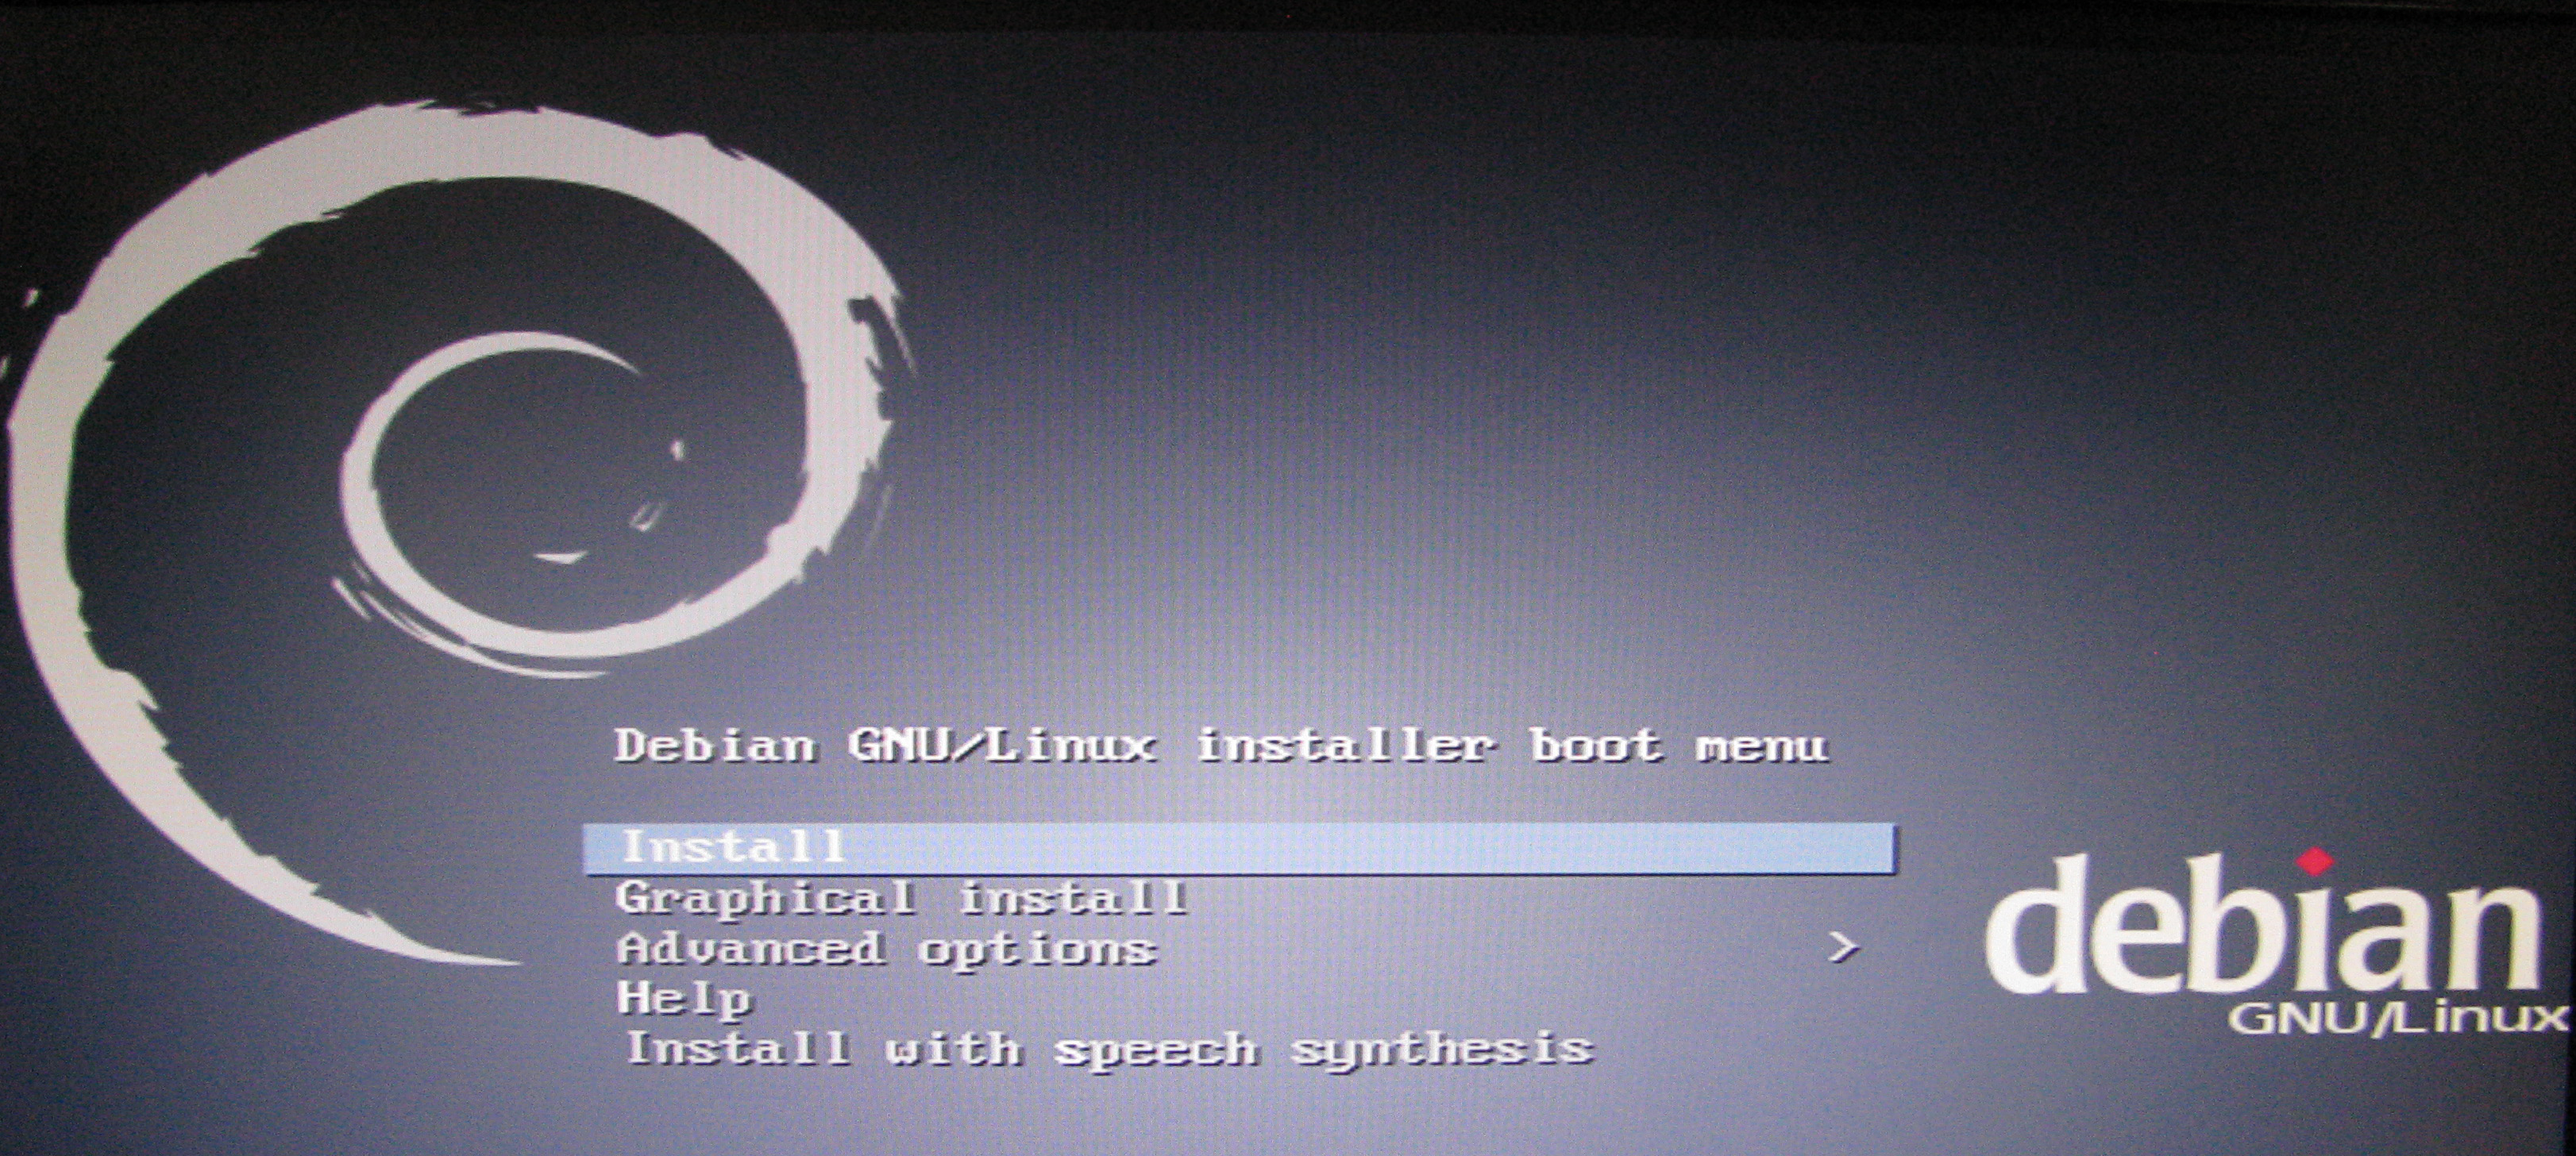
\includegraphics[width=0.45\textwidth]{bootmenu}
\caption{Je kiest hier de eerste optie \textbf{Install} met \texttt{enter}, om de installatie te beginnen. }
\label{fig:taal-keuze-scherm}
\end{figure}

Boot van de installatie CDROM. Je komt dan in een menu.
Je accepteert de eerste optie \textbf{Install} met \texttt{enter}.


\subsection{Localisatie instellingen}
\begin{figure}[H]
\centering
\includegraphics[width=0.45\textwidth]{taal-keuze-scherm}
\includegraphics[width=0.45\textwidth]{lokatie-keuze-scherm}
\caption{Taal en lokatie instellingen.}
\label{fig:taal-keuze-scherm}
\end{figure}

Op het volgende twee schermen, zie figuur~\ref{fig:taal-keuze-scherm},  moet je de taal kiezen; kies \textbf{Dutch} (pijltje omhoog en dan \texttt{enter}). In de scherm daarna, selecteer je  \textbf{Nederland} als land en drukt op \texttt{enter}. Vanaf gaan we niet meer zeggen dat je op \texttt{enter} moet drukken.

\begin{figure}[H]
\centering
\includegraphics[width=0.45\textwidth]{toetsenbord-indeling-scherm}
\caption{Kies hier \textbf{American English}.}
\label{fig:toetsenbord-indeling-scherm}
\end{figure}

Als toetsenbordindeling kies je \textbf{American English} (zie figuur~\ref{fig:toetsenbord-indeling-scherm}).


\subsection{Netwerk instellingen}
Je wacht tot de debian installer de aanvullende installatie modules heeft geladen. Het kan zijn dat er vragen komen over ontbrekende firmware. Die moet je allen met \textbf{nee} beantwoorden.

\begin{figure}[H]
\centering
\includegraphics[width=0.45\textwidth]{computernaam-scherm}
\includegraphics[width=0.45\textwidth]{domeinnaam-scherm}
\caption{Hostnaam en domeinnaam schermen.}
\label{fig:computernaam-scherm}
\end{figure}

Vul \textbf{debian} in als computernaam (figuur~\ref{fig:computernaam-scherm}).

En vul \textbf{lan} in bij domeinnaam.


\subsection{Gebruikers en wachtwoorden}

\begin{figure}[H]
\centering
\includegraphics[width=0.45\textwidth]{root-wachtwoord-scherm}
\includegraphics[width=0.45\textwidth]{root-wachtwoord-bevestiging}
\caption{Vul hier tweemaal \textbf{root} in.}
\label{fig:root-wachtwoord-scherm}
\end{figure}

Nu moeten het root wachtwoord worden gezet, zie figuur~\ref{fig:root-wachtwoord-scherm}.
Vul als root wachtwoord \textbf{root} in, en doe dit nogmaals ter controle.

\begin{figure}[H]
\centering
\includegraphics[width=0.45\textwidth]{nieuwe-gebruiker-naam}
\includegraphics[width=0.45\textwidth]{nieuwe-gebruiker-echte-naam}
\caption{Toevoegen van een nieuwe gebruiker.}
\label{fig:nieuwe-gebruiker}
\end{figure}

Je vult \textbf{Tux} in als volledige naam van de nieuwe aardse gebruiker (figuur~\ref{fig:nieuwe-gebruiker}).
De debian installer suggereert dan \textbf{tux} als gebruikersnaam.
Dat accepteer je met \texttt{enter}.

Als wachtwoord vul je \textbf{tux} in. Dit moet nog een keer worden bevestigd.


\subsection{Schijfindeling}
Bij de schijfindeling kies je \textbf{Begeleid - benut gehele schijf en gebruik LVM met encryptie}, zoals in figuur~\ref{fig:schijven-indelen}.
Nu kies je de schijf die moet worden ingedeeld; dit zal meestal geen keuze opleveren, omdat de meeste machines maar \'{e}\'{e}n schijf hebben.

\begin{figure}[H]
\centering
\includegraphics[width=0.45\textwidth]{schijven-indelen-scherm}
\includegraphics[width=0.45\textwidth]{schijf-uitkiezen-scherm}
\caption{Kies hier de optie met encryptie.}
\label{fig:schijven-indelen}
\end{figure}


Nu moet je kiezen hoe de schijf gaat worden opgedeeld (figuur~\ref{fig:aparte-partities}); je kiest de onderste optie \textbf{Afzondelijke /home, /usr, /var en /tmp partitie}.

\begin{figure}[H]
\centering
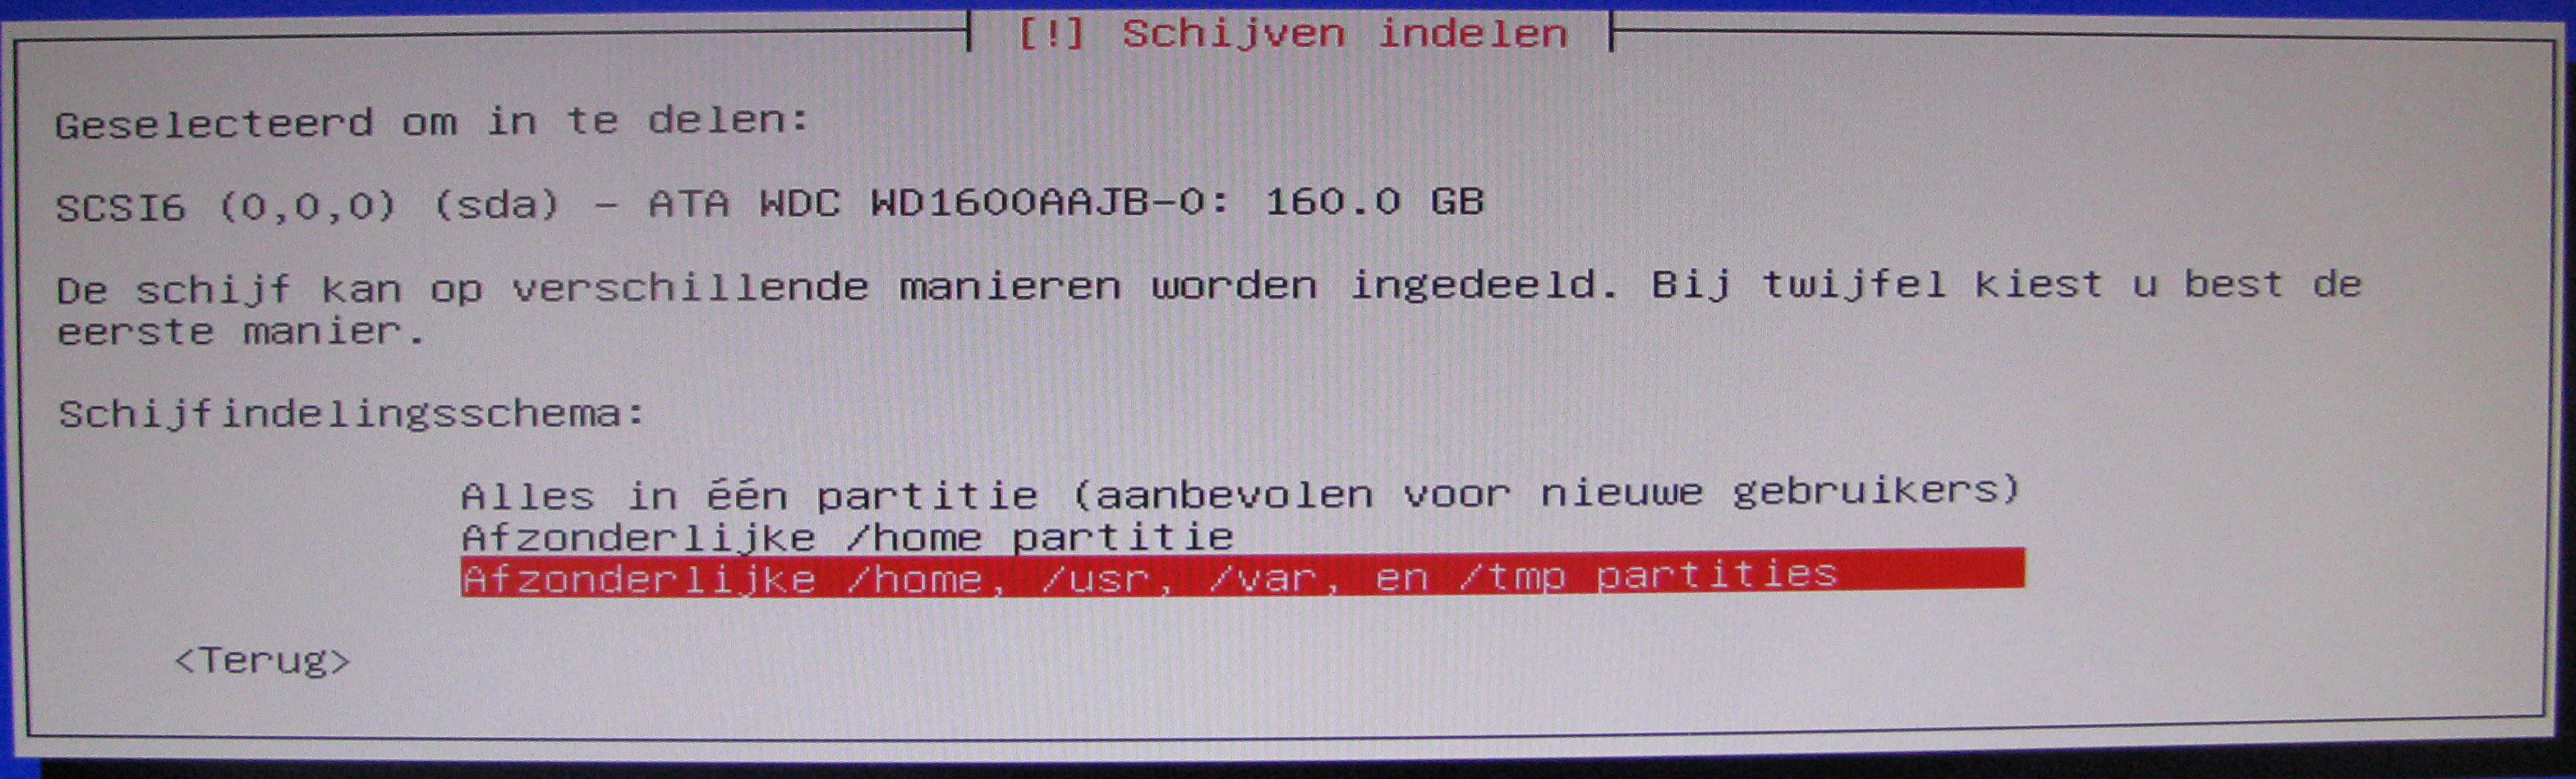
\includegraphics[width=0.45\textwidth]{schijf-indelen-afzonderlijke-partities}
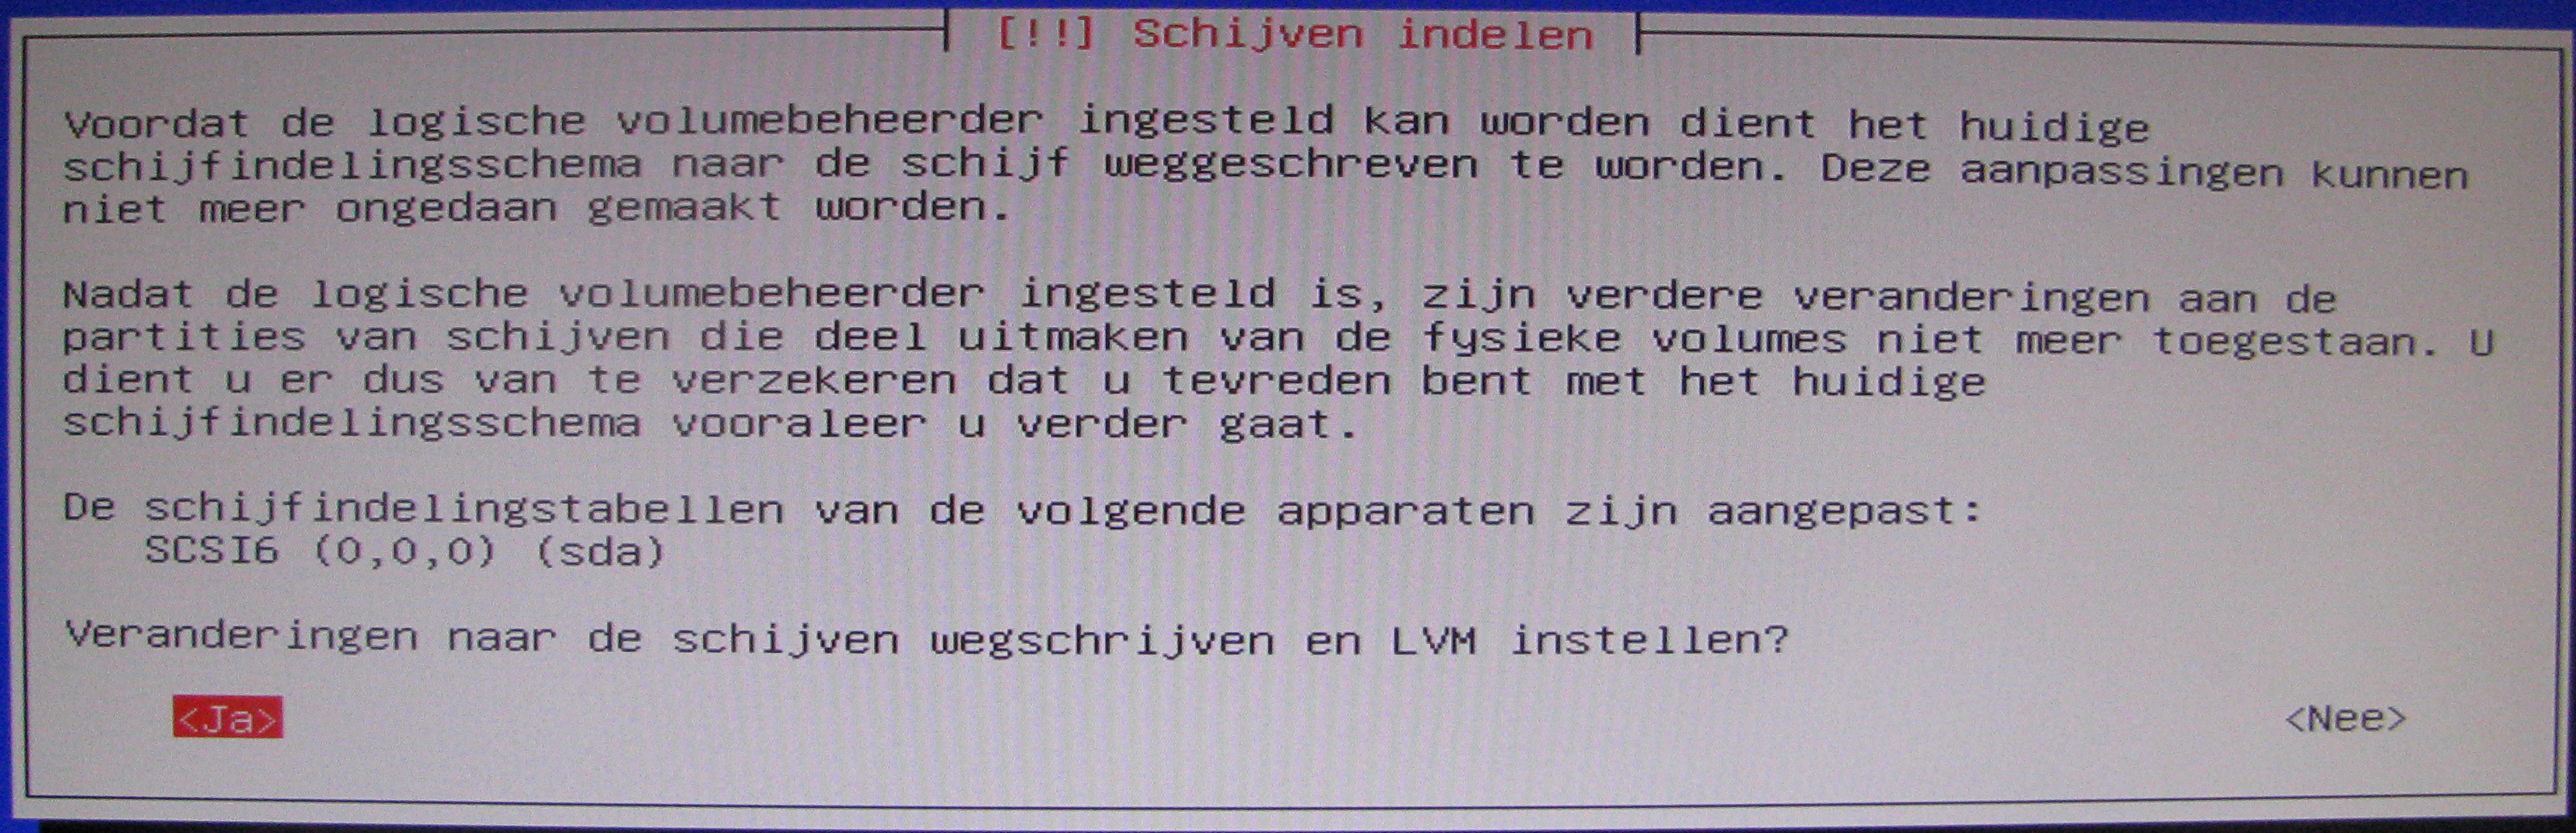
\includegraphics[width=0.45\textwidth]{lvm-instellen-scherm}
\caption{In de eerste scherm kiest je de onderste optie.}
\label{fig:aparte-partities}
\end{figure}


Nadat je dit bevestigd hebt, gaat de installer de gehele disk wissen (figuur~\ref{fig:schijf-wissen}), dat kan even duren (in de orde van uren). Je mag dit annuleren.

\begin{figure}[H]
\centering
\includegraphics[width=0.45\textwidth]{schijven-wissen-scherm}
\caption{Je mag dit annuleren.}
\label{fig:schijf-wissen}
\end{figure}

\begin{figure}[H]
\centering
\includegraphics[width=0.45\textwidth]{schijven-wachtwoordzin-scherm}
\includegraphics[width=0.45\textwidth]{schijven-wachtwoordzin-bevestiging}
\includegraphics[width=0.45\textwidth]{schijven-zwakke-wachtwoordzin}
\caption{Vul hier \textbf{gnu} in als wachtwoordzin.}
\label{fig:wachtwoordzin-scherm}
\end{figure}

Zoals in figuur~\ref{fig:wachtwoordzin-scherm} wordt er om een wachtwoordzin gevraagd, je vult \textbf{gnu} in.

Dit moet je nogmaals te controle doen.

Je moet nu bevestigen dat dit een zwakke wachtwoordzin is. 

\begin{figure}[H]
\centering
\includegraphics[width=0.45\textwidth]{schijven-overzicht-scherm}
\includegraphics[width=0.45\textwidth]{schijven-tweede-overzicht-scherm}
\caption{Bevestig tweemaal de gemaakte schijfindeling.}
\label{fig:schijven-overzicht}
\end{figure}


Het partitie schema wordt nog eenmaal aan je getoond (figuur~\ref{fig:schijven-overzicht}) met de mogelijkheid om wijzingen aan te brengen. Dat doe je niet, maar gaat verder.

Daarna wordt het nogmaals ter bevestiging getoond, opdat je het nog \'{e}\'{e}n keer kunt controleren. Je bevestigt de voorgestelde keuze.


\subsection{Pakketbeheer}

\begin{figure}[H]
\centering
\includegraphics[width=0.45\textwidth]{pakketbeheer-landkeuze-scherm}
\includegraphics[width=0.45\textwidth]{pakketbeheer-mirror-scherm}
\caption{Kies \textbf{Nederlands} als land van de Debian-archief-spiegelserver en als spiegelserver \textbf{ftp.nluug.nl}.}
\label{fig:pakketten}
\end{figure}

Zoals je in figuur~\ref{fig:pakketten} ziet moet je als land voor je Debian mirror \textbf{Nederland} kiezen en in het scherm daarop volgend kies je \textbf{ftp.nluug.nl}. 


Op de vraag die daarop volgt (figuur~\ref{fig:httpproxy}), waar je een HTTP-proxy moet kiezen druk je alleen \texttt{enter}.

\begin{figure}[H]
\centering
\includegraphics[width=0.45\textwidth]{pakketbeheer-proxy-scherm}
\caption{Hier laat je het invul veld leeg en drukt alleen op \texttt{enter}.}
\label{fig:httpproxy}
\end{figure}

Zoals in figuur~\ref{fig:popcon} te zien is willen wij meedoen aan de populariteits competitie. Hiermee laten wij aan de vrijwilligers van Debian weten welke programma eindgebruikers belangrijk vinden, opdat zij hun prioriteiten goed kunnen stellen.

\begin{figure}[H]
\centering
\includegraphics[width=0.45\textwidth]{populariteits-contest-scherm}
\caption{Je selecteert hier \textbf{ja}.}
\label{fig:popcon}
\end{figure}

\subsection{Software selectie}

\begin{figure}[H]
\centering
\includegraphics[width=0.45\textwidth]{software-selectie-scherm}
\label{fig:software-selectie-scherm}
\end{figure}

Nu volgt er een scherm (figuur~\ref{fig:software-selectie-scherm}) over de te installeren programma's. Omdat wij een aangepaste installatie doen, mag je hier alleen \textbf{Standaard systeemhulpmiddelen} aangevinkt laten. Je gaat met de pijltjestoetsen omhoog naar \textbf{Debian desktop environment} en vinkt deze uit met de spatiebalk. Dan navigeer je met \texttt{tab} naar \textbf{Volgende} en drukt op \texttt{enter}.

\subsection{Bootloader}

Je gaat mee in het voorstel van figuur~\ref{fig:grub} om GRUB in het masterboot record op te installeren.


\begin{figure}[H]
\centering
\includegraphics[width=0.45\textwidth]{grub-installatie-scherm}
\caption{Je laat GRUB in het masterboot record installeren}
\label{fig:grub}
\end{figure}

Nu rond je de installatie af zoals in figuur~\ref{fig:afronden}.

\begin{figure}[H]
\centering
\includegraphics[width=0.45\textwidth]{installatie-afronden-scherm}
\caption{Je leest de instructies, voert ze uit en kiest \textbf{Volgende}.}
\label{fig:afronden}
\end{figure}

\section{Debian Amsterdam specifieke installatie}

Omdat wij de het systeem hebben laten versleutelen moeten we bij het opstarten een wachtwoordzin opgeven om verder te gaan (figuur~\ref{fig:diskwachtwoord}).

\begin{figure}[H]
\centering
\includegraphics[width=0.45\textwidth]{diskwachtwoordzin-scherm}
\caption{Je typt hier \textbf{gnu}, gevolgd door \texttt{enter}. Merk op dat de karakters niet op het scherm verschijnen, ook niet als sterretjes.}
\label{fig:diskwachtwoord}
\end{figure}

Nu verschijnt het tekstlogin scherm van Linux. Dit noemen we een \textit{virtual terminal}. Volg de aanwijzingen van figuur~\ref{fig:loginprompt} op.

\begin{figure}[H]
\centering
\includegraphics[width=0.45\textwidth]{loginprompt-scherm}
\includegraphics[width=0.45\textwidth]{ingelogd-scherm}
\caption{Achter \textbf{debian login:} type je \textbf{root}, gevolgd door \texttt{enter}, dit is tevens het wachtwoord. Dus als \textbf{Password:} verschijnt type je weer \textbf{root}, gevolgd door \texttt{enter}.}
\label{fig:loginprompt}
\end{figure}

\subsection{Installatie van gekozen pakketten}

Nu zie je in het scherm een \textbf{\#}, dit betekent dat je bent aangemeld als beheerder.
Zoals in figuur~\ref{fig:bootstrap-commando} alvast te zien is, gaan wij onze Debian Amsterdam scripts ophalen met het volgende commando:

\begin{lstlisting}[language=bash]
wget --no-check-certificate -q -O- goo.gl/WHL7kR|sh
\end{lstlisting}
Ter verduidelijking de tekens: \texttt{-O-} bestaan uit 'min', 'hoofdletter O' en 'min'.

\begin{figure}[H]
\centering
\includegraphics[width=0.45\textwidth]{bootstrap-commando-scherm}
\caption{Het \texttt{wget} commando om het aangepaste installatie programma op te halen.}
\label{fig:bootstrap-commando}
\end{figure}

Het volgende commando dat wij geven zal een groot gedeelte van de installatie verder uitvoeren, helaas moet je er wel even bijblijven omdat er een paar vragen worden gesteld.

\begin{lstlisting}[language=bash]
install-debian.sh
\end{lstlisting}

\begin{figure}[H]
\centering
\includegraphics[width=0.45\textwidth]{install-debian-scherm}
\caption{We roepen hier het hoofdscript aan met \texttt{install-debian.sh}}
\label{fig:install-debian}
\end{figure}

De vraag die wordt gesteld is over het wachtwoord en volledige naam van de nieuwe gebruiker \textbf{tux}.

\begin{figure}[H]
\centering
\includegraphics[width=0.45\textwidth]{tux-wachtwoord-scherm}
\includegraphics[width=0.45\textwidth]{tux-volledige-naam-scherm}
\caption{Hier geef je als wachtwoord \textbf{tux}, gevolgd door \texttt{enter}. Dit moet je nog een keer doen en dan bij \textbf{Volledige naam []:} moet je \textbf{Tux} invullen. Daarna druk je op \texttt{enter} tot het script verder loopt.}
\label{fig:tuxinfo}
\end{figure}

Dan is het tijd om de extra pakketten te installeren met:
\begin{lstlisting}[language=bash]
install-nice-to-have.sh
\end{lstlisting}

\begin{figure}[H]
\centering
\includegraphics[width=0.45\textwidth]{install-nice-to-have-scherm}
\caption{Het commando voor de extra pakketten.}
\label{fig:nicetohave}
\end{figure}

